\documentclass{standalone}
\usepackage{tikz}
\usetikzlibrary{fit}
\usetikzlibrary{shapes.geometric}
\begin{document}
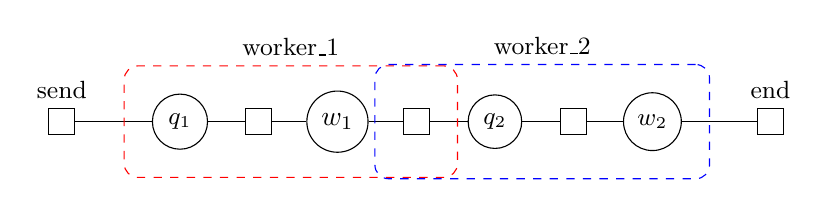
\begin{tikzpicture}[square/.style={regular polygon,regular polygon sides=4}, box/.style = {draw,red, dashed, inner sep=10pt,rounded corners=5pt}]

    \node[label={\small send}] at (-1.5, 0) [square, draw] (s_1) {};

    \node at (0, 0) [circle, minimum size = 0.7cm, draw] (q_1) {\small $q_1$}; 
    \node at (1, 0) [square, draw] (e_1) {};
    \node at (2, 0) [circle, draw] (w_1) {$w_1$};
    \node at (3, 0) [square, draw] (e_2) {};

    \node at (4, 0) [circle, draw] (q_2) {\small $q_2$};
    \node at (5, 0) [square, draw] (e_3) {};
    
    \node at (6, 0) [circle, draw] (w_2) {\small $w_2$};
    \node[label={\small end}] at (7.5, 0) [square, draw] (e_4) {};
    
    \draw (s_1.east) -- (q_1.west);
    \draw (q_1.east) -- (e_1.west);
    \draw (e_1.east) -- (w_1.west);
    \draw (w_1.east) -- (e_2.west);
    \draw (e_2.east) -- (q_2.west);
    \draw (q_2.east) -- (e_3.west);
    \draw (e_3.east) -- (w_2.west);
    \draw (w_2.east) -- (e_4.west);
    \node[label={\small worker\_1}, box, fit=(q_1)(e_2)] {};
    \node[label={\small worker\_2}, box, blue, fit=(e_2)(w_2)] {};
\end{tikzpicture}

\end{document}

